\section{Introduction}
\begin{figure}[ht]
  \centering
  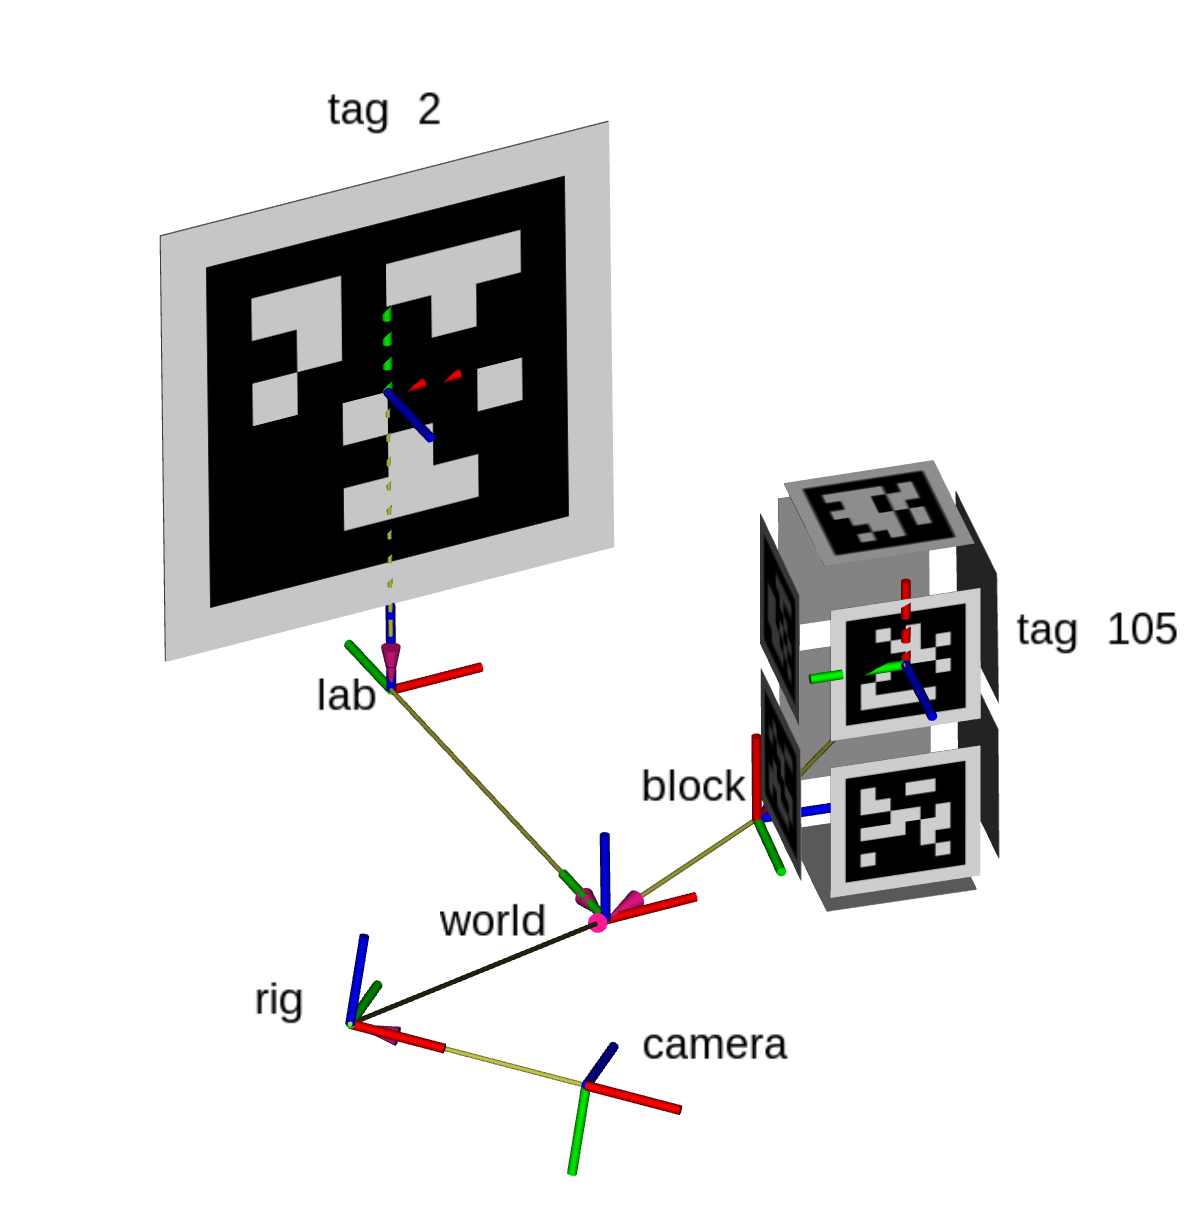
\includegraphics[width=\columnwidth]{scene_with_block.png}
  \caption{Single-camera TagSLAM scene with dynamic ``rig'' and ``block''
    bodies, and a static ``lab'' body.}
  \label{fig:scene_with_block}
\end{figure}

Accurate and robust Simultaneous Localization And Mapping (SLAM)
algorithms are arguably one of the corner pieces for building
autonomous systems. For this reason, SLAM has been studied extensively
since the 1980s, see Ref.\ \cite{cadena2016}. In this work, we will
focus our attention on graph based visual SLAM, and how to make it
more accessible for quantitative experiments in a controlled
environment.

In a nutshell, SLAM methods take sensor data such as camera images as
input and extract easily recognizable features (``landmarks''). The
landmarks are entered into a map such that when the same landmark is
detected again later, the observer's pose can be determined by
triangulation. In graph based SLAM, a nonlinear optimizer such as
GTSAM \cite{kaess2011} is used to simultaneously optimize the pose of
the observer and the location of the landmarks, given the sensor
measurements.

Despite intense research efforts \cite{cadena2016} SLAM still faces
several challenges:

{\em Recognizing previously seen landmarks (''loop closure'')}: This
is often difficult if landmarks are observed from a different
viewpoint, or under different lighting conditions. TagSLAM sidesteps
this issue by requiring that AprilTag visual markers \cite{wang2016}
with unique identifiers be placed in view of a camera. This clearly
comes at the cost of increased experimental setup effort, and being
restricted to controlled environments, where tags can be placed.

{\em Maintaining a map of landmarks}: In an effort to limit memory
consumption and achieve fast retrieval, landmarks must be at some
point discarded, efficient retrieval databases must be updated and
queried, adding considerable complexity \cite{murartal2016}. If loop
closure fails, the estimated camera pose starts to drift, which is a
well-known problem with local-map-only algorithms such as
visual-inertial odometry (VIO). Since TagSLAM operates only with a set
of fewer than 1000 tags, memory and retrieval speed are not an
issue. Additionally, by measuring tag distances or coordinates with
e.g. a laser based device, it is possible to introduce additional
metric constraints into the optimization process. Finally, specifying
the pose of at least one tag explicitly allows for tying the SLAM map
to a known world map.

{\em Poor initialization}: A bad starting guess can cause the
non-linear optimizer employed for graph based SLAM to fail or converge
to a local minima. Since TagSLAM's back end is based on a such an
optimizer \cite{kaess2011}, this difficulty must be addressed. Here we
present a detailed description of how we achieve robust initialization
to make TagSLAM a tool that can be applied to a wide range of
real-world test cases without parameter tuning.

It is worthwhile noting that SLAM is a rather general algorithm, and
therefore can solve several related, simpler problems as well. If for
example the camera pose is known, one can estimate the pose of the
landmarks. Likewise, if a map of the landmarks is known, the camera
pose can be inferred. TagSLAM inherits all of this flexibility. In
contrast to traditional SLAM packages however, where moving landmarks
are filtered out, TagSLAM can explicitly model and track multiple
objects that have tags attached to them. This means TagSLAM can also
be used for pose estimation of objects other than cameras, as shown in
Fig. \ref{fig:scene_with_block}.  TagSLAM's robustness and
availability as an open-source ROS \cite{quigley2009} package make it
particularly accessible for researchers new to robotics. It is now
being used at UPenn's GRASP lab for extrinsic camera calibration with
non-overlapping views, loop closure on visual-inertial odometry
benchmarks, tag mapping, object pose estimation, and more.
